%%%%%%%%%%%%%%%%%%%%%%%%%%%%%%%%%%%%%%%%%
% University Assignment Title Page 
% LaTeX Template
% Version 1.0 (27/12/12)
%
% This template has been downloaded from:
% http://www.LaTeXTemplates.com
%
% Original author:
% WikiBooks (http://en.wikibooks.org/wiki/LaTeX/Title_Creation)
%
% License:
% CC BY-NC-SA 3.0 (http://creativecommons.org/licenses/by-nc-sa/3.0/)
%
%%%%%%%%%%%%%%%%%%%%%%%%%%%%%%%%%%%%%%%%%
%\title{Title page with logo}
%----------------------------------------------------------------------------------------
%	PACKAGES AND OTHER DOCUMENT CONFIGURATIONS
%----------------------------------------------------------------------------------------

\documentclass[12pt]{article}
\usepackage[english]{babel}
\usepackage[utf8]{inputenc}
\usepackage{natbib}
\usepackage{amsmath}
\usepackage{color}
\usepackage[explicit]{titlesec}
\usepackage[hyphens,spaces,obeyspaces]{url}
\usepackage{graphicx}
\usepackage{caption}
\usepackage{subcaption}
\usepackage{grffile}

\begin{document}

\begin{titlepage}

\newcommand{\HRule}{\rule{\linewidth}{0.5mm}} % Defines a new command for the horizontal lines, change thickness here

\center % Center everything on the page
 
%----------------------------------------------------------------------------------------
%	HEADING SECTIONS
%----------------------------------------------------------------------------------------

\textsc{\LARGE University of St Andrews}\\[1.5cm] % Name of your university/college
\textsc{\Large Distributed Systems}\\[0.5cm] % Major heading such as course name
\textsc{\large CS4103}\\[0.5cm] % Minor heading such as course title

%----------------------------------------------------------------------------------------
%	TITLE SECTION
%----------------------------------------------------------------------------------------

\HRule \\[0.4cm]
{ \huge \bfseries Ring-Based Distributed System}\\[0.4cm] % Title of your document
\HRule \\[1.5cm]
 
%----------------------------------------------------------------------------------------
%	AUTHOR SECTION
%----------------------------------------------------------------------------------------


\Large \emph{Author:}\\
 \textsc{150008022}\\[1cm] % Your name
 
%----------------------------------------------------------------------------------------
%	DATE SECTION
%----------------------------------------------------------------------------------------

{\large \today}\\[2cm] % Date, change the \today to a set date if you want to be precise

%----------------------------------------------------------------------------------------
%	LOGO SECTION
%---------------------------------------------------------------------------------------


\includegraphics[width = 4cm]{images/standrewslogo.png}
 
%----------------------------------------------------------------------------------------

\vfill % Fill the rest of the page with whitespace

\end{titlepage}

\section*{Goal}

To demonstrate an understanding of leader election and mutual exclusion in distributed systems by developing a ring-based distributed social media application.

\tableofcontents
\newpage

\pagenumbering{arabic}
\setcounter{page}{1} 

\section{Initial Set-up}

Java 8 was chosen for this project due to it's friendly socket API, and Maven \cite{maven} was used as the build tool. TDD was implemented with JUnit4 as the the test suite framework.

The project was started with the intention of implementing the bully algorithm, as it provided fault tolerance with low overhead. 

\subsection{Configuration}

Since each node would be running on an isolated machine, the planned testing environment would involve using \emph{ssh} to start the nodes remotely. Providing the configuration as command line arguments was considered simpler than other methods, and was implemented using the Apache Commons CLI library \cite{apachecli}.

\subsection{Communication}
TCP was used for communication \textbf{around} the ring for the following reasons:
\begin{enumerate}
    \item Reliable communication.
    \item Keepalive functionality allows effective failure detection.
    \item Connection is reused frequently between predecessors and successors, justifying handshake overhead.
\end{enumerate}

UDP was used for communication \textbf{across} the ring for the following reasons:
\begin{enumerate}
    \item Reliable communication.
    \item Keepalive functionality allows effective failure detection.
    \item Connection is reused frequently between predecessors and successors, justifying handshake overhead.
\end{enumerate}


\begin{figure}[!h]
\centering
\begin{subfigure}{.5\textwidth}
  \centering
  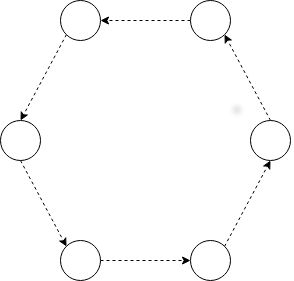
\includegraphics[width=.6\linewidth]{images/tcp}
  \caption{TCP Around Ring}
  \label{fig:sub1}
\end{subfigure}%
\begin{subfigure}{.5\textwidth}
  \centering
  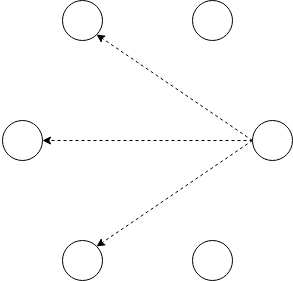
\includegraphics[width=.6\linewidth]{images/udp}
  \caption{UDP Across Ring}
  \label{fig:sub2}
\end{subfigure}
\caption{The different types of communication used}
\label{fig:test}
\end{figure}

\section{Leader/Coordinator Election}

\section{Receive/Send Posts}

\bibliographystyle{unsrt}
\bibliography{mybib}

\end{document}
